\documentclass[a4paper]{scrartcl}
\usepackage[cm]{fullpage}
\usepackage{amsmath, amssymb, esint}
\usepackage{tikz}

\usepackage{sectsty}
\sectionfont{\large\selectfont}
\subsectionfont{\normalsize\selectfont}

\usepackage{siunitx}

\begin{document}

\title{PHYS2113: Assignment 1}
\author{ \\ \\ }
\date{2016-04-03}
\maketitle

\section{A particle of mass \(m\) is subject to a force \(F(x) = k x\), with \(k > 0\). The particle is initially at rest at position \(x = x_0\). Find the position of the particle as a function of time, i.e. \(x(t)\) (1 mark)}
\[F(x) = m \ddot{x} = k x\]
\[\therefore \ddot{x} - \frac{k}{m} x = 0\]
which has the characteristic equation:
\[A^2 - \frac{k}{m} = 0\]
\[\therefore A = \pm\sqrt\frac{k}{m}\]
\[\therefore x(t) = C_1 e^{\sqrt\frac{k}{m} t} + C_2 e^{-\sqrt\frac{k}{m} t}\]
Given the initial conditions:
\[x(0) = C_1 + C_2 = x_0\]
\[\dot{x}(0) = C_1 - C_2 = 0\]
Solving for the constants and substituting back in yields:
\[x(t) = \frac{x_0}{2} \left(e^{\sqrt\frac{k}{m} t} + e^{-\sqrt\frac{k}{m} t}\right)\]

\section{An archer decides to shoot an apple from a tree with a bow and arrow, a horizontal distance \(L\) away and a vertical distance \(h\) above him. He aims the bow directly at the apple. However at the moment he releases the arrow, at speed \(V\), the apple drops off the tree. Show that the arrow will still strike the falling apple. You may neglect air resistance. (1 mark)}
Taking the initial position of the arrow to be the origin:
\begin{align*}
    \ddot{\mathbf{r}}_{arrow} &= \begin{pmatrix} 0 \\ -g \end{pmatrix} \\
    \dot{\mathbf{r}}_{arrow}(t = 0) &= \frac{1}{\sqrt{L^2 + h^2}}\begin{pmatrix} V L \\ V h \end{pmatrix} \\
    \mathbf{r}_{arrow}(t = 0) &= \begin{pmatrix} 0 \\ 0 \end{pmatrix} \\
    \therefore \mathbf{r}_{arrow} &= \begin{pmatrix} \frac{V L t}{\sqrt{L^2 + h^2}} \\ \frac{V h t}{\sqrt{L^2 + h^2}} - \frac{1}{2} g t^2 \end{pmatrix}
\end{align*}
\begin{align*}
    \ddot{\mathbf{r}}_{apple} &= \begin{pmatrix} 0 \\ -g \end{pmatrix} \\
    \dot{\mathbf{r}}_{apple}(t = 0) &= \begin{pmatrix} 0 \\ 0 \end{pmatrix} \\
    \mathbf{r}_{apple}(t = 0) &= \begin{pmatrix} L \\ h \end{pmatrix} \\
    \therefore \mathbf{r}_{apple} &= \begin{pmatrix} L \\ h - \frac{1}{2} g t^2 \end{pmatrix}
\end{align*}
Solving \(\mathbf{r}_{arrow}(t = t_c) = \mathbf{r}_{apple}(t = t_c)\) for a candidate time \(t_c\), we find:
\[t_c = \frac{\sqrt{L^2 + h^2}}{V}\]
\[\mathbf{r}_{arrow}(t_c) = \begin{pmatrix} L \\ h - \frac{g (L^2 + h^2)}{2 V^2} \end{pmatrix} = \mathbf{r}_{apple}(t_c)\]
Thus the arrow will strike the apple at time \(t_c\).

\section{A wheel of radius \(R\) is rolling along a smooth, horizontal table at a constant angular velocity \(\omega\). The path travelled by any point on the rim of the wheel as it rolls in a straight line is called a cycloid. If \(\theta\) is the angular position of a marked point on the rim at time \(t\) that is initially vertical at time \(t = 0\), then: (1.5 marks)}
\begin{center}
    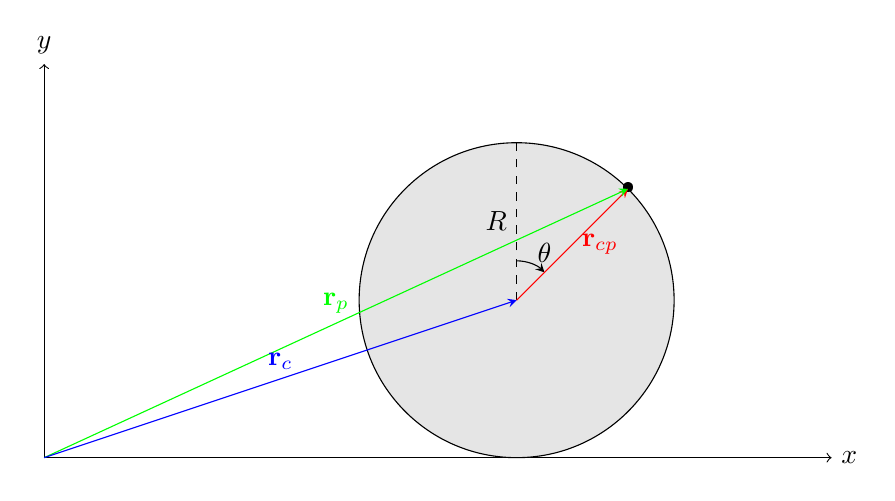
\begin{tikzpicture}
        \draw [->] (0, 0) -- (10, 0) node [right] {\(x\)};
        \draw [->] (0, 0) -- (0, 5) node [above] {\(y\)};
        \draw [fill = white!80!gray] (6, 2) circle (2);
        \draw ({6 + sqrt(2)}, {2 + sqrt(2)}) node {\textbullet};
        \draw [dashed] (6, 2) -- (6, 4) node [midway, left] {\(R\)};
        \draw [-stealth] (6, 2.5) arc (90:45:0.5) node [above] {\(\theta\)};
        \draw [-stealth, red] (6, 2) -- ({6 + sqrt(2)}, {2 + sqrt(2)}) node [midway, right] {\(\mathbf{r}_{cp}\)};
        \draw [-stealth, green] (0, 0) -- ({6 + sqrt(2)}, {2 + sqrt(2)}) node [midway, above] {\(\mathbf{r}_{p}\)};
        \draw [-stealth, blue] (0, 0) -- (6, 2) node [midway, above] {\(\mathbf{r}_c\)};
    \end{tikzpicture}

    (Not to scale)
\end{center}

\subsection{Show that the position of the centre of the wheel is given by, in Cartesian coordinates, \(\mathbf{r}_c = (R \theta, R)\), with respect to the origin.}
From the given information:
\begin{align*}
    \theta_0 &= 0 \\
    \mathbf{r}_c(t = 0) &= \begin{pmatrix} 0 \\ R \end{pmatrix}
\end{align*}
The centre is always \(R\) above the \(x\)-axis since the wheel is on the axis. The circle rolls on the \(x\)-axis, so it travels its arc length in the \(x\) direction, which is given by \(R \theta\).
\[\therefore \mathbf{r}_c = \begin{pmatrix} R \theta \\ R \end{pmatrix}\]

\subsection{Show that the position of the marked point on the rim is \(\mathbf{r}_{cp} = (R \sin \theta, R \cos \theta)\), with respect to the centre of the wheel.}
\begin{center}
    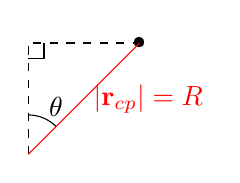
\begin{tikzpicture}
        \draw ({6 + sqrt(2)}, {2 + sqrt(2)}) node {\textbullet};
        \draw [dashed] (6, 2) -- (6, {2 + sqrt(2)}) -- ({6 + sqrt(2)}, {2 + sqrt(2)});
        \draw (6 + 0.2, {2 + sqrt(2)}) -- (6 + 0.2, {2 + sqrt(2) - 0.2}) -- (6, {2 + sqrt(2) - 0.2});
        \draw (6, 2.5) arc (90:45:0.5) node [above] {\(\theta\)};
        \draw [red] (6, 2) -- ({6 + sqrt(2)}, {2 + sqrt(2)}) node [midway, right] {\(|\mathbf{r}_{cp}| = R\)};
    \end{tikzpicture}
\end{center}
Using simple trigonometry on a right angle triangle with \(\theta\) being one of the included angles, it is clear that:
\[\mathbf{r}_{cp} = \begin{pmatrix} R \sin \theta \\  R \cos \theta \end{pmatrix}\]

\subsection{Hence determine the position of the marked point with respect to the origin; i.e. the path of the cycloid.}
\[\mathbf{r}_{p} = \mathbf{r}_{c} + \mathbf{r}_{cp} = R \begin{pmatrix} \theta + \sin \theta \\  1 + \cos \theta \end{pmatrix} = R \begin{pmatrix} \omega t + \sin \omega t \\  1 + \cos \omega t \end{pmatrix}\]

\subsection{The find the velocity \(\mathbf{v}(t)\) and acceleration \(\mathbf{a}(t)\) of the marked point in these coordinates.}
\[\mathbf{v}(t) = \frac{\mathrm{d}\mathbf{r}_p}{\mathrm{d}t} = \omega R \begin{pmatrix} 1 + \cos \omega t \\ - \sin \omega t \end{pmatrix}\]
\[\mathbf{a}(t) = \frac{\mathrm{d}\mathbf{v}}{\mathrm{d}t} = -\omega^2 R \begin{pmatrix} \sin \omega t \\ \cos \omega t \end{pmatrix}\]

\subsection{At the instant the marked point is at the top of the wheel find the radius of curvature \(S\) of its path.}
\[S = \frac{|\mathbf{v}|^3}{|\mathbf{v} \times \mathbf{a}|} = 4 R \left|\cos\left(\frac{\theta}{2}\right)\right|\]
At the top of the wheel, \(\theta = 0\):
\[S\big|_{\theta = 0} = 4 R\]

\section{Two beads of mass \(m\) are initially at rest at the top of a frictionless hoop of mass \(M\) and radius \(R\), which stands vertically on a horizontal table, as in the diagram. The beads are given tiny kicks and slide in opposite directions around the hoop. They are attached to the hoop, so cannot fall off. What is the largest value of \(\frac{m}{M}\) for which the hoop never rises up from the ground? (1.5 marks)}
\begin{center}
    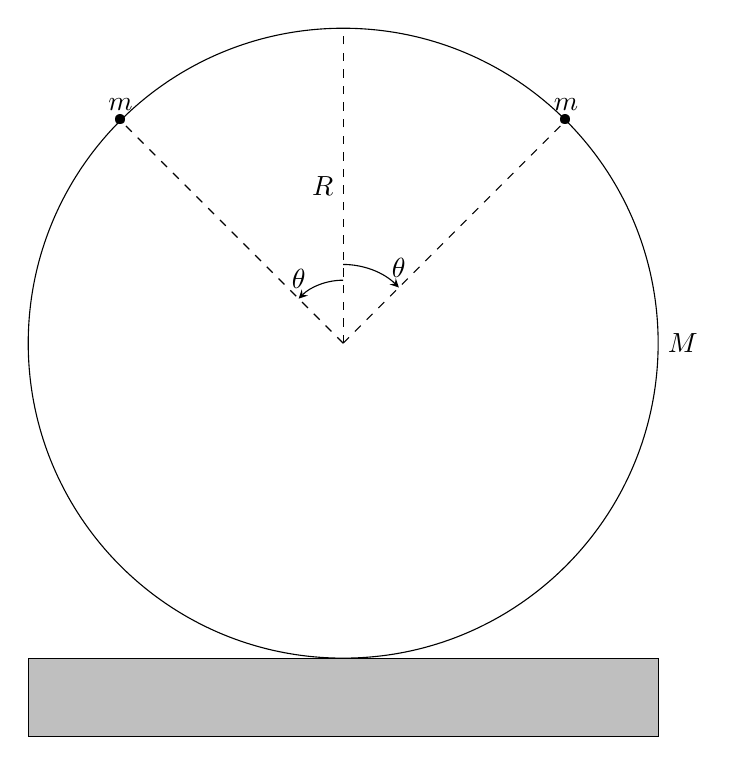
\begin{tikzpicture}
        \draw (0, 0) circle (4);
        \draw (4, 0) node [right] {\(M\)};
        \draw ({2 * sqrt(2)}, {2 * sqrt(2)}) node {\textbullet} node [above] {\(m\)};
        \draw (-{2 * sqrt(2)}, {2 * sqrt(2)}) node {\textbullet} node [above] {\(m\)};
        \draw [dashed] (0, 0) -- (0, 4) node [midway, left] {\(R\)};
        \draw [-stealth] (0, 1) arc (90:45:1) node [above] {\(\theta\)};
        \draw [-stealth] (0, 0.8) arc (90:135:0.8) node [above] {\(\theta\)};
        \draw [dashed] (0, 0) -- ({2 * sqrt(2)}, {2 * sqrt(2)});
        \draw [dashed] (0, 0) -- ({-2 * sqrt(2)}, {2 * sqrt(2)});
        \draw [fill = white!50!gray] (-4, -4) rectangle (4, -5);
    \end{tikzpicture}
\end{center}

First consider only the mass to the right. It will have a centripetal force of:
\[-\mathbf{F}_r = \frac{m v^2}{R} = m g \cos \theta - \mathbf{N}_r\]
where \(\mathbf{N}\) is the normal reaction force, which only exists in the radial direction.

Using the conservation of energy and our initial conditions:
\begin{align*}
    \Delta KE &= \Delta PE \\
    \frac{1}{2} m v^2 &= m g R (1 - \cos \theta)
\end{align*}

Combining the equations yields the normal reaction force \(\mathbf{N}\):
\[\mathbf{N}_r = m g (3 \cos \theta - 2)\]

By Newton's 3rd law, the normal force on the hoop is equal an opposite to \(\mathbf{N}\), and by symmetry from the mass on the left, the horizontal components cancel while verticals add, so we are only left with the vertical component from both masses as:
\[-2 \mathbf{N}_r \cos \theta = 2 m g (2 - 3 \cos \theta) \cos \theta\]

Since we require the hoop to never rise, this force must be no greater than the gravitational force on the hoop. Rearranging for \(\frac{m}{M}\) and then maximising (noting that only positive values are valid) will give the answer we are looking for. That is:
\[2 m g (2 - 3 \cos \theta) \cos \theta \leq M g\]
\[\frac{m}{M} \leq \frac{1}{4 \cos \theta - 6 \cos^2 \theta}\]
\[\max\left(\frac{m}{M}\right) = \min\left(\frac{1}{4 \cos \theta - 6 \cos^2 \theta}\right) = \frac{3}{2}\]

\end{document}
